\documentclass[aspectratio=169,10pt]{beamer}
\usetheme{metropolis}
\usepackage{amsmath,amssymb,bm}
\usepackage{siunitx}
\usepackage{booktabs}
\usepackage[table]{xcolor}
\usepackage{tikz}
\usetikzlibrary{arrows.meta,calc,positioning,patterns}
\usepackage{pgfplots}
\pgfplotsset{compat=1.17}
\sisetup{per-mode=symbol,detect-all}
\metroset{numbering=fraction,progressbar=frametitle,block=fill}
\tikzset{capt/.style={text width=5.2cm,align=center}}
\hypersetup{colorlinks=true,urlcolor=blue!60!black,linkcolor=.}
\addtobeamertemplate{frametitle}{}{%
  \begin{tikzpicture}[remember picture,overlay]
    \node[anchor=north east,yshift=-1.5pt,xshift=-6pt] at (current page.north east) {
\includegraphics[height=0.7cm]{logos/itu_logo_beyaz.pdf}};
  \end{tikzpicture}}
\titlegraphic{\hfill
\includegraphics[height=1.6cm]{logos/itu_logo_laci.pdf}}

\title{Lecture 7: Butt and Fillet Welds}
\subtitle{UCK 364E Design of Machine Elements}
\author{Prof.\ Dr.\ Onur Tunçer}
\institute{Department of Aeronautical Engineering, Istanbul Technical University}
\date{Fall 2026}

\begin{document}
\maketitle

\begin{frame}{Today}
\begin{enumerate}
  \item Why the perfect joint is not used to hold an airliner together
  \item What welding does to the metal --- and why steel and aluminium go opposite ways
  \item Joints, welds, and the symbol on the drawing
  \item Butt welds
  \item Fillet welds: the throat, and the convention everyone uses
  \item Static strength --- weld metal, and the parent beside it
  \item Fatigue: the toe decides
  \item Defects, inspection, and why welding is a special process
  \item Where to put a weld
\end{enumerate}
\end{frame}

\section{Why this lecture exists}

\begin{frame}{A joint with no hole}
Every joint in Lectures 5 and 6 had a hole, and the hole set the strength.

\medskip
A weld has none. It can develop the \alert{full section}, it is light, leak-tight and cheap.

\vfill
So why is an airliner riveted?
\begin{enumerate}
  \item \textbf{A weld changes the material.} Beside every weld, the alloy and temper you specified are gone.
  \item \textbf{A weld creates its own notch.} In fatigue the toe --- not the alloy --- sets the life.
  \item \textbf{A weld is continuous.} A crack has an unbroken path. The Liberty ships taught this.
  \item \textbf{A weld cannot be verified by measurement.} Quality has to be built in.
\end{enumerate}
\end{frame}

\begin{frame}{Where welding lives in aerospace}
Where its advantages are decisive and its problems can be managed:
\begin{itemize}
  \item steel-tube trusses and \alert{engine mounts} --- Project 1
  \item landing-gear and engine parts, heat treated \emph{after} welding
  \item exhaust systems and hot ducting
  \item pressure vessels and propellant tanks
\end{itemize}
\vfill
\begin{block}{Three questions for every weld}
For a bolt you asked: how strong is the fastener, how strong is the plate?\\
For a weld: how strong is the \textbf{weld metal}, how strong is the \textbf{parent beside it now},
and --- if the load varies --- \textbf{what shape is the toe}.
\end{block}
\end{frame}

\section{What welding does to the metal}

\begin{frame}{Three zones, and a heat treatment nobody specified}
\centering
\resizebox{!}{0.78\textheight}{% A fusion weld in section, and what happens to hardness across it.
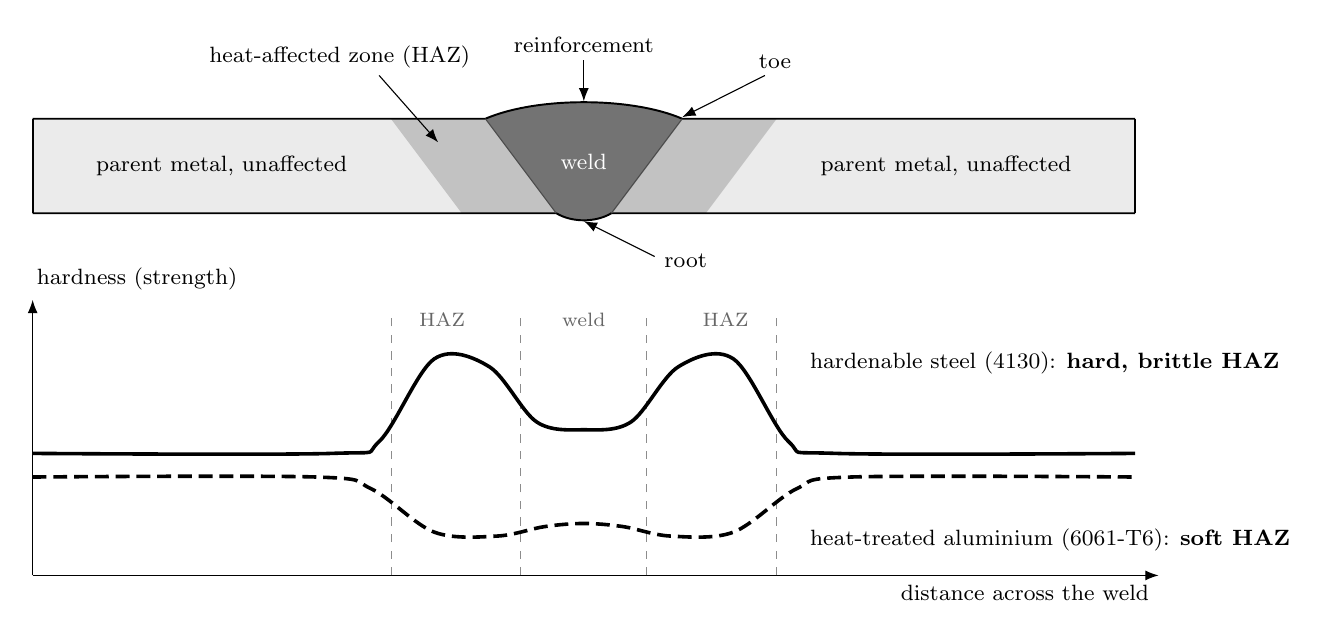
\begin{tikzpicture}[>=Latex,line join=round]
\tikzset{lab/.style={font=\footnotesize}, sm/.style={font=\scriptsize}}
% ---- section ----
\fill[black!8] (-7,0) rectangle (7,1.2);
\fill[black!24] (-0.35,0) -- (-1.25,1.2) -- (-2.45,1.2) -- (-1.55,0) -- cycle;
\fill[black!24] (0.35,0) -- (1.25,1.2) -- (2.45,1.2) -- (1.55,0) -- cycle;
\fill[black!55] (-0.35,0) -- (-1.25,1.2) .. controls (-0.6,1.48) and (0.6,1.48) .. (1.25,1.2) -- (0.35,0) .. controls (0.15,-0.12) and (-0.15,-0.12) .. cycle; % weld metal
\draw[line width=0.7pt] (-7,0) -- (-0.35,0) .. controls (-0.15,-0.12) and (0.15,-0.12) .. (0.35,0) -- (7,0) (-7,1.2) -- (-1.25,1.2) .. controls (-0.6,1.48) and (0.6,1.48) .. (1.25,1.2) -- (7,1.2);
\draw[line width=0.7pt] (-7,0) -- (-7,1.2) (7,0) -- (7,1.2);
\draw[black!70,line width=0.4pt] (-0.35,0) -- (-1.25,1.2) (0.35,0) -- (1.25,1.2);
\node[lab,text=white] at (0,0.65) {weld};
\node[lab] at (-4.6,0.6) {parent metal, unaffected}; \node[lab] at (4.6,0.6) {parent metal, unaffected};
\draw[<-,line width=0.4pt] (-1.85,0.9) -- (-2.6,1.75); \node[lab,anchor=south] at (-3.1,1.72) {heat-affected zone (HAZ)};
\draw[<-,line width=0.4pt] (1.25,1.22) -- (2.3,1.75); \node[lab,anchor=south west] at (2.1,1.72) {toe};
\draw[<-,line width=0.4pt] (0,-0.1) -- (0.9,-0.55); \node[lab,anchor=west] at (0.9,-0.6) {root};
\draw[<-,line width=0.4pt] (0,1.42) -- (0,1.95); \node[lab,anchor=south] at (0,1.92) {reinforcement};
% ---- hardness traverse ----
\begin{scope}[yshift=-4.6cm]
\draw[->] (-7,0) -- (7.3,0) node[lab,anchor=north east] {distance across the weld};
\draw[->] (-7,0) -- (-7,3.5) node[lab,anchor=south west,xshift=-2pt] {hardness (strength)};
\foreach \x in {-2.45,-0.8,0.8,2.45}{\draw[black!45,dashed,line width=0.3pt] (\x,0) -- (\x,3.3);}
\node[sm,black!60] at (-1.8,3.25) {HAZ}; \node[sm,black!60] at (1.8,3.25) {HAZ}; \node[sm,black!60] at (0,3.25) {weld};
% steel: hard HAZ
\draw[line width=1.3pt] plot[smooth,tension=0.55] coordinates {(-7,1.55) (-3.2,1.55) (-2.6,1.7) (-1.9,2.75) (-1.2,2.65) (-0.6,1.95) (0,1.85) (0.6,1.95) (1.2,2.65) (1.9,2.75) (2.6,1.7) (3.2,1.55) (7,1.55)};
\node[lab,anchor=west] at (2.75,2.7) {hardenable steel (4130): \textbf{hard, brittle HAZ}};
% aluminium: soft HAZ
\draw[line width=1.3pt,dash pattern=on 5pt off 2.5pt] plot[smooth,tension=0.55] coordinates {(-7,1.25) (-3.4,1.25) (-2.7,1.1) (-1.9,0.55) (-1.1,0.5) (-0.5,0.62) (0,0.66) (0.5,0.62) (1.1,0.5) (1.9,0.55) (2.7,1.1) (3.4,1.25) (7,1.25)};
\node[lab,anchor=west] at (2.75,0.45) {heat-treated aluminium (6061-T6): \textbf{soft HAZ}};
\end{scope}
\end{tikzpicture}
}
\end{frame}

\begin{frame}{Steel and aluminium go opposite ways}
\begin{columns}[T]
\begin{column}{0.48\textwidth}
\textbf{Hardenable steel (4130, 4340)}

\medskip
The HAZ is heated past transformation, then quenched by the cold metal around it.

\medskip
Result: \alert{harder and brittle} --- untempered martensite --- and prone to cracking, worse with
hydrogen.

\medskip
Cure: control the cooling; for a heat-treated part, weld first, \emph{then} heat treat the assembly.
\end{column}
\begin{column}{0.48\textwidth}
\textbf{Heat-treated aluminium (6061-T6, 2xxx, 7xxx)}

\medskip
The temper is a fine precipitate grown over hours. Welding heat destroys it in seconds.

\medskip
Result: \alert{softer}. 6061-T6: \SI{290}{MPa} as bought, about \SI{165}{MPa} across a weld.

\medskip
Cure: re-solution-treat and age --- or design to the welded strength.
\end{column}
\end{columns}
\end{frame}

\begin{frame}{Why airframes are riveted and rockets are welded}
\textbf{2024 and 7075 are not fusion weldable in practice.} They crack as the weld freezes, and
what survives has lost its temper. That, more than tradition, is why Lecture 6 was about rivets.

\vfill
\textbf{A propellant tank is different.} It must be leak-tight, it is nearly all membrane, and the
alloy can be chosen to weld (2219, 2195).
\begin{itemize}
  \item The weld sits on a \alert{weld land}: a locally thickened strip.
  \item \alert{Friction stir welding} joins without melting --- a rotating tool stirs the edges
        together in the solid state. It is how current launch-vehicle tanks are made.
\end{itemize}
\end{frame}

\begin{frame}{The processes you will meet}
\centering\footnotesize
\begin{tabular}{@{}lll@{}}
\toprule
\textbf{Process} & \textbf{Heat source} & \textbf{Where you meet it}\\
\midrule
TIG (GTAW, 141) & tungsten arc, inert gas, hand-fed filler & \textbf{the aerospace standard}: tube clusters, thin sheet\\
MIG / MAG (GMAW) & arc from a consumable wire & structural work, ground equipment\\
Manual metal arc (SMAW) & coated stick electrode & structural steel; Shigley's E60xx--E120xx\\
Electron beam, laser & focused beam, deep and narrow & precision engine and gear parts\\
Resistance spot, seam & current through clamped sheets & lightly loaded sheet assemblies\\
Friction stir (FSW) & none: solid-state stirring & aluminium tanks and panels\\
\bottomrule
\end{tabular}
\end{frame}

\section{Joints, welds, and the symbol}

\begin{frame}{Five joints, two welds}
\centering
\resizebox{0.9\textwidth}{!}{% The five joint types, and the two weld types that make them.
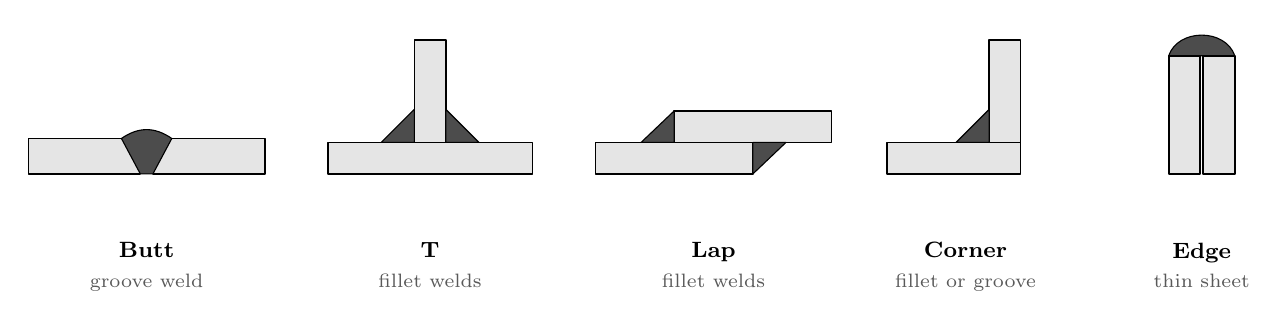
\begin{tikzpicture}[line join=round]
\tikzset{pl/.style={fill=black!10,draw=black,line width=0.6pt}, wd/.style={fill=black!70,draw=black,line width=0.4pt},
  ttl/.style={font=\footnotesize\bfseries,anchor=north}, sub/.style={font=\scriptsize,anchor=north,text=black!65,align=center}}
% butt
\begin{scope}
 \path[pl] (-1.5,0) rectangle (-0.08,0.45); \path[pl] (0.08,0) rectangle (1.5,0.45);
 \path[wd] (-0.08,0) -- (-0.32,0.45) .. controls (-0.1,0.6) and (0.1,0.6) .. (0.32,0.45) -- (0.08,0) -- cycle;
 \node[ttl] at (0,-0.75) {Butt}; \node[sub] at (0,-1.15) {groove weld};
\end{scope}
% T
\begin{scope}[xshift=3.6cm]
 \path[pl] (-1.3,0) rectangle (1.3,0.4); \path[pl] (-0.2,0.4) rectangle (0.2,1.7);
 \path[wd] (-0.2,0.4) -- (-0.62,0.4) -- (-0.2,0.82) -- cycle; \path[wd] (0.2,0.4) -- (0.62,0.4) -- (0.2,0.82) -- cycle;
 \node[ttl] at (0,-0.75) {T}; \node[sub] at (0,-1.15) {fillet welds};
\end{scope}
% lap
\begin{scope}[xshift=7.2cm]
 \path[pl] (-1.5,0) rectangle (0.5,0.4); \path[pl] (-0.5,0.4) rectangle (1.5,0.8);
 \path[wd] (-0.5,0.4) -- (-0.92,0.4) -- (-0.5,0.8) -- cycle; \path[wd] (0.5,0.4) -- (0.92,0.4) -- (0.5,0) -- cycle;
 \node[ttl] at (0,-0.75) {Lap}; \node[sub] at (0,-1.15) {fillet welds};
\end{scope}
% corner
\begin{scope}[xshift=10.6cm]
 \path[pl] (-1.2,0) rectangle (0.5,0.4); \path[pl] (0.1,0.4) rectangle (0.5,1.7);
 \path[wd] (0.1,0.4) -- (-0.32,0.4) -- (0.1,0.82) -- cycle;
 \node[ttl] at (-0.2,-0.75) {Corner}; \node[sub] at (-0.2,-1.15) {fillet or groove};
\end{scope}
% edge
\begin{scope}[xshift=13.4cm]
 \path[pl] (-0.42,0) rectangle (-0.02,1.5); \path[pl] (0.02,0) rectangle (0.42,1.5);
 \path[wd] (-0.42,1.5) .. controls (-0.3,1.85) and (0.3,1.85) .. (0.42,1.5) -- cycle;
 \node[ttl] at (0,-0.75) {Edge}; \node[sub] at (0,-1.15) {thin sheet};
\end{scope}
\end{tikzpicture}
}

\vfill\raggedright
\begin{itemize}
  \item A \textbf{groove (butt) weld}, fully penetrated, \emph{replaces the section}. The load flows
        straight through. \alert{The weld you want.}
  \item A \textbf{fillet weld} sits in a corner. The load turns a corner to get through it, and the
        unfused root is a built-in crack. \alert{The weld you can afford.}
\end{itemize}
\end{frame}

\begin{frame}{The weld symbol --- you specify, you do not draw the bead}
\centering
\resizebox{0.88\textwidth}{!}{% Anatomy of a weld symbol (ISO 2553), with the joint it describes.
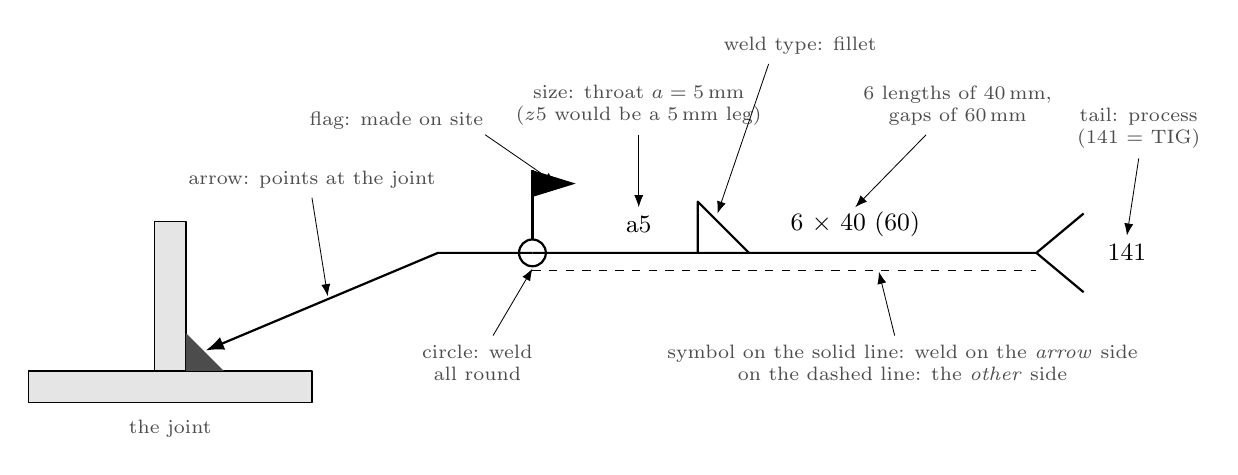
\begin{tikzpicture}[>=Latex,line join=round]
\tikzset{lab/.style={font=\footnotesize}, sm/.style={font=\scriptsize,text=black!70}, pl/.style={fill=black!10,draw=black,line width=0.6pt}}
% ---- the joint ----
\path[pl] (-6.2,-0.4) rectangle (-2.6,0); \path[pl] (-4.6,0) rectangle (-4.2,1.9);
\fill[black!70] (-4.2,0) -- (-3.72,0) -- (-4.2,0.48) -- cycle;
\node[sm,anchor=north] at (-4.4,-0.5) {the joint};
% ---- the symbol ----
\draw[line width=0.8pt,->] (0.2,1.5) -- (-1.0,1.5) -- (-3.95,0.26);
\draw[line width=0.8pt] (0.2,1.5) -- (6.6,1.5) -- (7.2,2.0) (6.6,1.5) -- (7.2,1.0);
\draw[line width=0.5pt,dashed] (0.2,1.28) -- (6.6,1.28);
\draw[line width=0.8pt] (2.3,1.5) -- (2.3,2.15) -- (2.95,1.5);            % fillet symbol on the arrow side
\node[font=\small] at (1.55,1.86) {a5}; \node[font=\small] at (4.3,1.86) {6 $\times$ 40 (60)}; \node[font=\small] at (7.75,1.5) {141};
\draw[line width=0.8pt] (0.2,1.5) circle[radius=0.17];                    % weld all round
\draw[line width=0.8pt] (0.2,1.67) -- (0.2,2.55); \fill (0.2,2.55) -- (0.75,2.38) -- (0.2,2.21) -- cycle; % site weld
% ---- callouts ----
\draw[<-,line width=0.3pt] (-2.4,0.95) -- (-2.6,2.2); \node[sm,anchor=south] at (-2.6,2.2) {arrow: points at the joint};
\draw[<-,line width=0.3pt] (1.55,2.08) -- (1.55,3.0); \node[sm,anchor=south,align=center] at (1.55,3.0) {size: throat $a=\SI{5}{mm}$\\ ($z5$ would be a \SI{5}{mm} leg)};
\draw[<-,line width=0.3pt] (2.55,2.0) -- (3.2,3.9); \node[sm,anchor=south,align=center] at (3.6,3.9) {weld type: fillet};
\draw[<-,line width=0.3pt] (4.3,2.08) -- (5.2,3.0); \node[sm,anchor=south,align=center] at (5.6,3.0) {6 lengths of \SI{40}{mm},\\ gaps of \SI{60}{mm}};
\draw[<-,line width=0.3pt] (7.75,1.72) -- (7.9,2.7); \node[sm,anchor=south,align=center] at (7.9,2.7) {tail: process\\ (141 = TIG)};
\draw[<-,line width=0.3pt] (0.2,1.3) -- (-0.3,0.45); \node[sm,anchor=north,align=center] at (-0.5,0.45) {circle: weld\\ all round};
\draw[<-,line width=0.3pt] (0.5,2.38) -- (-0.4,3.0); \node[sm,anchor=south east,align=right] at (-0.3,2.95) {flag: made on site};
\draw[<-,line width=0.3pt] (4.6,1.26) -- (4.8,0.45); \node[sm,anchor=north,align=center] at (4.9,0.45) {symbol on the solid line: weld on the \emph{arrow} side\\ on the dashed line: the \emph{other} side};
\end{tikzpicture}
}

\vfill\footnotesize\raggedright
ISO 2553 shown. The American system (AWS A2.4) gives the fillet size as the \emph{leg} and has no
dashed line: below the line is the arrow side, above is the other side.
\end{frame}

\begin{frame}{Throat or leg --- say which}
\begin{columns}[c]
\begin{column}{0.5\textwidth}
A fillet is sized by its throat $a$ or its leg $z$:
\[ a = 0.707\,z \]
A ``5 mm fillet'' is therefore \alert{two different welds}. One has twice the weld metal of the other.

\medskip
ISO drawings: \textbf{a5} or \textbf{z7}. Write the letter.

\medskip
Shigley and American practice use the leg, and call it $h$. So do we: $h$ for the leg, $a$ for the throat.
\end{column}
\begin{column}{0.46\textwidth}
\centering
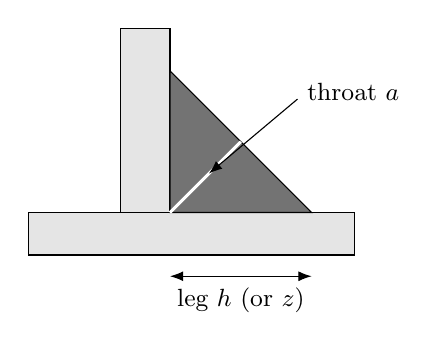
\begin{tikzpicture}[>=Latex,scale=0.9]
\fill[black!10] (-2.0,-0.6) rectangle (2.6,0); \draw (-2.0,-0.6) rectangle (2.6,0);
\fill[black!10] (-0.7,0) rectangle (0,2.6); \draw (-0.7,0) rectangle (0,2.6);
\fill[black!55] (0,0) -- (2,0) -- (0,2) -- cycle; \draw (0,0) -- (2,0) -- (0,2) -- cycle;
\draw[white,line width=1.1pt] (0,0) -- (1,1);
\draw[<->] (0,-0.9) -- (2,-0.9); \node[font=\small,anchor=north] at (1,-0.92) {leg $h$ (or $z$)};
\draw[<-] (0.55,0.55) -- (1.8,1.6); \node[font=\small,anchor=west] at (1.8,1.7) {throat $a$};
\end{tikzpicture}
\end{column}
\end{columns}
\end{frame}

\section{Butt welds}

\begin{frame}{Butt welds}
Full penetration, plate thickness $t$, width $l$:
\[ \sigma=\frac{F}{t\,l}\qquad\qquad \tau=\frac{V}{t\,l} \]
The throat is the plate thickness.

\vfill
\begin{alertblock}{The reinforcement does not count}
The bulge above the surface adds no strength --- the plate beside it is still only $t$ thick. What
it adds is a \textbf{toe}. Harmless statically; in fatigue it is the problem. The best butt welds
are ground flush.
\end{alertblock}

\vfill
A \textbf{partial-penetration} butt weld is a different object: the unfused root is a crack across
the load, and the load path is eccentric. Not used in tension in anything that matters.
\end{frame}

\section{Fillet welds}

\begin{frame}{The fillet, and the plane it fails on}
\centering
\resizebox{0.92\textwidth}{!}{% Fillet weld: the names, and the throat plane of a transverse fillet.
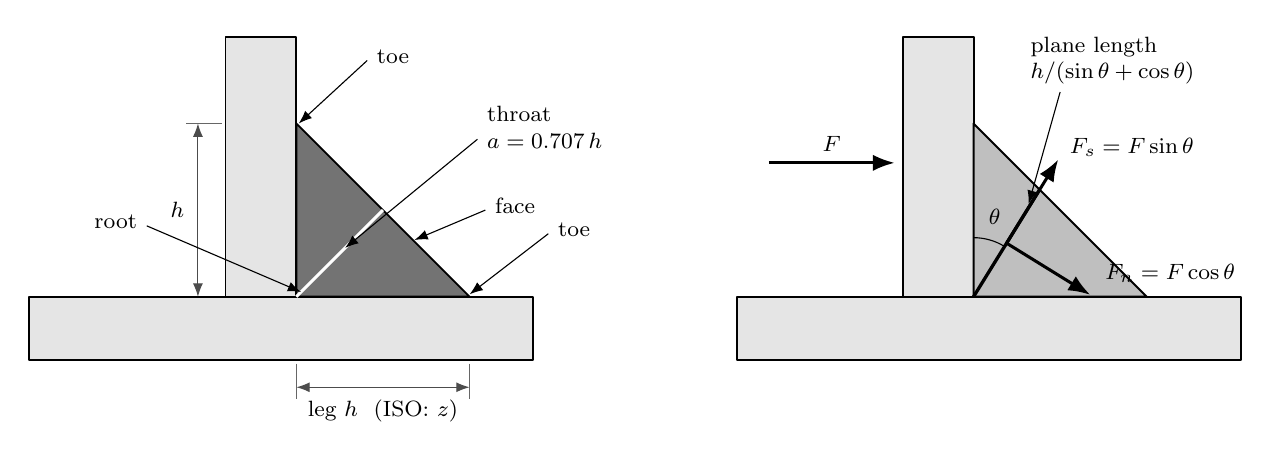
\begin{tikzpicture}[>=Latex,line join=round]
\tikzset{pl/.style={fill=black!10,draw=black,line width=0.7pt}, lab/.style={font=\footnotesize}, dimn/.style={<->,black!70,line width=0.4pt}}
% ---------- geometry ----------
\path[pl] (-3.4,-0.8) rectangle (3.0,0); \path[pl] (-0.9,0) rectangle (0,3.3);
\fill[black!55] (0,0) -- (2.2,0) -- (0,2.2) -- cycle; \draw[line width=0.7pt] (0,0) -- (2.2,0) -- (0,2.2) -- cycle;
\draw[white,line width=1.1pt] (0,0) -- (1.1,1.1);
\draw[dimn] (0,-1.15) -- (2.2,-1.15); \draw[black!60,line width=0.3pt] (2.2,-0.85) -- (2.2,-1.3) (0,-0.85) -- (0,-1.3);
\node[lab,anchor=north] at (1.1,-1.18) {leg $h$ \ (ISO: $z$)};
\draw[dimn] (-1.25,0) -- (-1.25,2.2); \draw[black!60,line width=0.3pt] (-0.95,2.2) -- (-1.4,2.2); \node[lab,anchor=east] at (-1.3,1.1) {$h$};
\draw[<-,line width=0.4pt] (0.62,0.62) -- (2.3,2.0); \node[lab,anchor=west,align=left] at (2.3,2.15) {throat\\ $a=0.707\,h$};
\draw[<-,line width=0.4pt] (2.2,0.03) -- (3.2,0.8); \node[lab,anchor=west] at (3.2,0.85) {toe};
\draw[<-,line width=0.4pt] (0.03,2.2) -- (0.9,3.0); \node[lab,anchor=west] at (0.9,3.05) {toe};
\draw[<-,line width=0.4pt] (0.06,0.06) -- (-1.9,0.9); \node[lab,anchor=east] at (-1.9,0.95) {root};
\draw[<-,line width=0.4pt] (1.5,0.72) -- (2.4,1.1); \node[lab,anchor=west] at (2.4,1.15) {face};
% ---------- throat plane at angle theta ----------
\begin{scope}[xshift=8.6cm]
\path[pl] (-0.9,0) rectangle (0,3.3); \path[pl] (-3.0,-0.8) rectangle (3.4,0);
\draw[line width=0.7pt,fill=black!25] (0,0) -- (2.2,0) -- (0,2.2) -- cycle;
% cut plane through the root at theta from the vertical leg
\draw[line width=1.2pt] (0,0) -- (0.84,1.36);
\draw[line width=0.4pt] (0,0.75) arc[start angle=90,end angle=58.3,radius=0.75]; \node[lab] at (0.27,1.02) {$\theta$};
\draw[->,line width=1.1pt] (-2.6,1.7) -- (-1.0,1.7); \node[lab,anchor=south] at (-1.8,1.72) {$F$};
\draw[->,line width=1.1pt] (0.42,0.68) -- ++(-31.7:1.25);
\draw[->,line width=1.1pt] (0.42,0.68) -- ++(58.3:1.25);
\node[lab,anchor=south west] at (1.1,1.66) {$F_s=F\sin\theta$};
\node[lab,anchor=west] at (1.55,0.3) {$F_n=F\cos\theta$};
\node[lab,anchor=west,align=left] at (0.6,3.0) {plane length\\ $h/(\sin\theta+\cos\theta)$};
\draw[<-,line width=0.4pt] (0.7,1.18) -- (1.1,2.6);
\end{scope}
\end{tikzpicture}
}
\end{frame}

\begin{frame}{The stress on the throat plane}
Cut a transverse fillet through the root at angle $\theta$. Plane length
$h/(\sin\theta+\cos\theta)$:
\[ \tau=\frac{F}{h\,l}\,\sin\theta\,(\sin\theta+\cos\theta),\qquad
   \sigma=\frac{F}{h\,l}\,\cos\theta\,(\sin\theta+\cos\theta) \]
\begin{itemize}
  \item shear is greatest at $\theta=\ang{67.5}$: \ $\tau_{\max}=1.207\,F/(hl)$
  \item von Mises is greatest at $\theta=\ang{62.5}$: \ $\sigma'=2.16\,F/(hl)$
\end{itemize}
\vfill
\alert{Nobody designs with these.} The real stress peaks at the root and the toe; this free body
is only a model.
\end{frame}

\begin{frame}{The design convention}
\begin{block}{Whatever the direction of the load}
Divide the force by the throat area, and call the result a shear stress:
\[ \tau=\frac{F}{0.707\,h\,l}=\frac{1.414\,F}{h\,l} \]
\end{block}
\begin{itemize}
  \item For a parallel fillet: the true average shear on the throat.
  \item For a transverse fillet: overstates the maximum shear by \SI{17}{\percent} (1.414 against 1.207).
  \item Ignores the normal stress and the stress concentration --- and makes up for both in the allowable.
\end{itemize}
\end{frame}

\begin{frame}{Parallel and transverse fillets do not work together}
\centering
\resizebox{0.86\textwidth}{!}{% A lap joint seen from above: parallel (longitudinal) and transverse fillets.
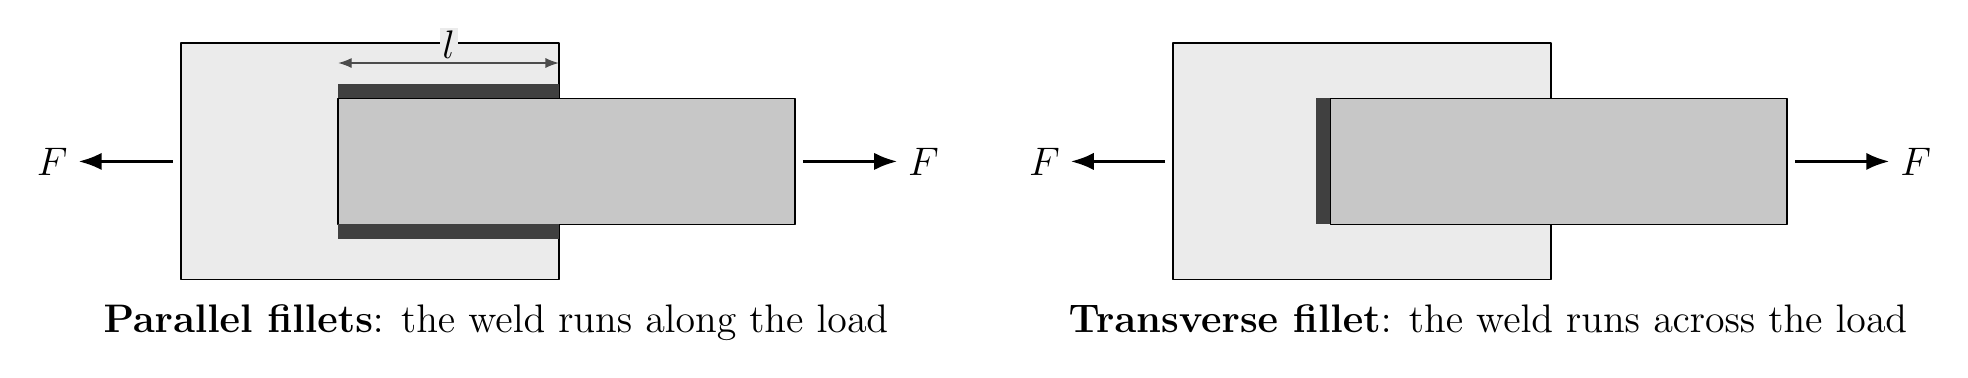
\begin{tikzpicture}[>=Latex,line join=round]
\tikzset{lab/.style={font=\Large}}
\begin{scope}
\fill[black!8] (-3.6,-1.5) rectangle (1.2,1.5); \draw[line width=0.6pt] (-3.6,-1.5) rectangle (1.2,1.5);
\fill[black!22] (-1.6,-0.8) rectangle (4.2,0.8); \draw[line width=0.6pt] (-1.6,-0.8) rectangle (4.2,0.8);
\fill[black!75] (-1.6,0.8) rectangle (1.2,0.98); \fill[black!75] (-1.6,-0.8) rectangle (1.2,-0.98);
\draw[->,line width=1.2pt] (4.3,0) -- (5.5,0) node[lab,anchor=west] {$F$};
\draw[->,line width=1.2pt] (-3.7,0) -- (-4.9,0) node[lab,anchor=east] {$F$};
\draw[<->,black!70,line width=0.4pt] (-1.6,1.25) -- (1.2,1.25); \node[lab,anchor=south,fill=black!8,inner sep=1pt] at (-0.2,1.27) {$l$};
\node[lab,anchor=north] at (0.4,-1.7) {\textbf{Parallel fillets}: the weld runs along the load};
\end{scope}
\begin{scope}[xshift=12.6cm]
\fill[black!8] (-3.6,-1.5) rectangle (1.2,1.5); \draw[line width=0.6pt] (-3.6,-1.5) rectangle (1.2,1.5);
\fill[black!22] (-1.6,-0.8) rectangle (4.2,0.8); \draw[line width=0.6pt] (-1.6,-0.8) rectangle (4.2,0.8);
\fill[black!75] (-1.78,-0.8) rectangle (-1.6,0.8);
\draw[->,line width=1.2pt] (4.3,0) -- (5.5,0) node[lab,anchor=west] {$F$};
\draw[->,line width=1.2pt] (-3.7,0) -- (-4.9,0) node[lab,anchor=east] {$F$};
\node[lab,anchor=north] at (0.4,-1.7) {\textbf{Transverse fillet}: the weld runs across the load};
\end{scope}
\end{tikzpicture}
}

\vfill\raggedright
A transverse fillet is about \alert{half as strong again} as a parallel one --- but deforms far
less before it breaks.
\begin{itemize}
  \item The convention is safe for both.
  \item A joint with both kinds does \emph{not} use them together: the stiff one breaks first.
        Same lesson as mixing rivets and bolts.
  \item Along a parallel fillet the \alert{ends} carry more than the middle. Weld ends are where
        cracks start.
\end{itemize}
\end{frame}

\section{Static strength}

\begin{frame}{Weld metal: match or overmatch}
The filler should be at least as strong as what it joins, so a good butt weld breaks in the plate.

\vfill
\centering\footnotesize
\begin{tabular}{@{}lccc@{}}
\toprule
\textbf{Electrode} & $S_{ut}$, MPa & $S_y$, MPa & Elong., \%\\
\midrule
E60xx & 427 & 345 & 17--25\\
E70xx & 482 & 393 & 22\\
E80xx & 551 & 462 & 19\\
E90xx & 620 & 531 & 14--17\\
E100xx & 689 & 600 & 13--16\\
E120xx & 827 & 737 & 14\\
\bottomrule
\end{tabular}
\qquad
\begin{tabular}{@{}lll@{}}
\toprule
\textbf{Loading} & \textbf{Weld} & \textbf{Allowable}\\
\midrule
Tension & butt & $0.60\,S_y$\\
Bearing & butt & $0.90\,S_y$\\
Bending & butt & $0.60$--$0.66\,S_y$\\
Compression & butt & $0.60\,S_y$\\
Shear & butt or fillet & $0.30\,S_{ut}$ (weld metal)\\
\bottomrule
\end{tabular}

\vfill\raggedright\normalsize
Shigley, Tables 9--3 and 9--4. \alert{Check the parent metal too}: in shear along the leg,
$0.40\,S_y$.
\end{frame}

\begin{frame}{Example 7.1 --- a bar lap-welded with two parallel fillets}
$60\times\SI{8}{mm}$ bar, $S_y=\SI{355}{MPa}$. Two fillets, $h=\SI{6}{mm}$, $l=\SI{75}{mm}$, E70xx.

\medskip
\begin{tabular}{@{}lll@{}}
\textbf{Weld metal} & $0.30\times482=\SI{145}{MPa}$ on $2(0.707)(6)(75)=\SI{636}{mm^2}$ & \alert{\SI{92}{kN}}\\[3pt]
Parent, shear along the legs & $0.40\times355=\SI{142}{MPa}$ on \SI{900}{mm^2} & \SI{128}{kN}\\[3pt]
The bar in tension & $0.60\times355=\SI{213}{MPa}$ on \SI{480}{mm^2} & \SI{102}{kN}\\
\end{tabular}

\vfill
The weld governs, at \SI{90}{\percent} of the bar.

\medskip
To develop the bar: $l=102\,000/(2\times0.707\times6\times145)=\SI{83}{mm}$.

\medskip
\alert{Eight millimetres of weld} on each side is the difference between a joint that is the weak
link and one that is not.
\end{frame}

\begin{frame}{In aerospace alloys, it is the parent metal that governs}
\textbf{Welded 4130 tube, not heat treated afterwards} --- the normal state of a tube truss.

\medskip
\centering
\begin{tabular}{@{}ll@{}}
\toprule
Normalised tube, away from any weld & $F_{tu}\approx\SI{655}{MPa}$ \ (\SI{95}{ksi})\\
Beside a weld at $30^\circ$ or less to the axis & $F_{tu}=\SI{620}{MPa}$ \ (\SI{90}{ksi})\\
Beside any other weld & $F_{tu}=\SI{552}{MPa}$ \ (\SI{80}{ksi})\\
\bottomrule
\end{tabular}

\vfill\raggedright\footnotesize
MIL-HDBK-5 section 8.2 values, quoted as classroom figures --- take the current MMPDS for real work.

\normalsize\vfill
\begin{block}{No fitting factor on a weld}
CS/FAR 25.625 excuses ``joints made under approved practices and based on comprehensive test
data'' --- and names welded joints. The price is the phrase \emph{approved practices}.
\end{block}
\end{frame}

\begin{frame}{Why the angle matters}
\centering
\resizebox{0.95\textwidth}{!}{% Three ways to join a 4130 tube end, and why the angle of the weld matters.
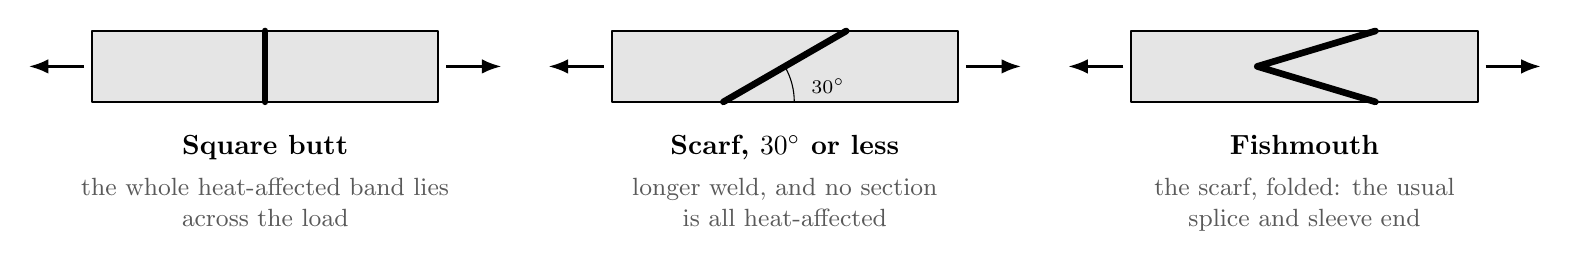
\begin{tikzpicture}[line join=round,>=Latex]
\tikzset{tb/.style={fill=black!10,draw=black,line width=0.7pt}, wl/.style={black,line width=2.4pt,line cap=round},
  ttl/.style={font=\normalsize\bfseries,anchor=north}, sub/.style={font=\small,anchor=north,text=black!65,align=center}}
\begin{scope}
 \path[tb] (-2.2,0) rectangle (2.2,0.9); \draw[wl] (0,0) -- (0,0.9);
 \draw[->,line width=0.9pt] (2.3,0.45) -- (3.0,0.45); \draw[->,line width=0.9pt] (-2.3,0.45) -- (-3.0,0.45);
 \node[ttl] at (0,-0.3) {Square butt}; \node[sub] at (0,-0.85) {the whole heat-affected band lies\\ across the load};
\end{scope}
\begin{scope}[xshift=6.6cm]
 \path[tb] (-2.2,0) rectangle (2.2,0.9); \draw[wl] (-0.78,0) -- (0.78,0.9);
 \draw[line width=0.4pt] (-0.78,0) ++(0.9,0) arc[start angle=0,end angle=30,radius=0.9]; \node[font=\scriptsize] at (0.55,0.2) {$30^\circ$};
 \draw[->,line width=0.9pt] (2.3,0.45) -- (3.0,0.45); \draw[->,line width=0.9pt] (-2.3,0.45) -- (-3.0,0.45);
 \node[ttl] at (0,-0.3) {Scarf, $30^\circ$ or less}; \node[sub] at (0,-0.85) {longer weld, and no section\\ is all heat-affected};
\end{scope}
\begin{scope}[xshift=13.2cm]
 \path[tb] (-2.2,0) rectangle (2.2,0.9);
 \draw[wl] (0.9,0.9) -- (-0.6,0.45) -- (0.9,0);
 \draw[->,line width=0.9pt] (2.3,0.45) -- (3.0,0.45); \draw[->,line width=0.9pt] (-2.3,0.45) -- (-3.0,0.45);
 \node[ttl] at (0,-0.3) {Fishmouth}; \node[sub] at (0,-0.85) {the scarf, folded: the usual\\ splice and sleeve end};
\end{scope}
\end{tikzpicture}
}

\vfill\raggedright
A square butt puts the whole heat-affected band across the load at one station.

A scarf or a fishmouth spreads it along the tube --- and is worth \SI{10}{ksi}.
\end{frame}

\begin{frame}{Example 7.2 --- a welded 4130 tube in tension}
$25.4\times\SI{0.889}{mm}$ tube, limit load \SI{20}{kN}. \ $A=\pi(D-t)t=\SI{68.5}{mm^2}$. \ Ultimate \SI{30}{kN}.

\vfill
\centering
\begin{tabular}{@{}llll@{}}
\toprule
Section & $F_{tu}$, MPa & Strength, kN & Margin\\
\midrule
Tube, away from the weld & 655 & 44.8 & $+0.49$\\
At a square-cut welded end & 552 & 37.8 & \alert{$+0.26$}\\
At a $30^\circ$ fishmouth end & 620 & 42.4 & $+0.41$\\
\bottomrule
\end{tabular}

\vfill\raggedright
The weld costs \SI{16}{\percent} of the tube cut square, \SI{5}{\percent} fishmouthed.

\medskip
The margin you report is the one \alert{at the weld} --- and the choice is made with a hacksaw,
before the torch is lit.
\end{frame}

\begin{frame}{Example 7.3 --- how thick must a weld land be?}
6061-T6 panel, \SI{4}{mm}, butt-welded, not re-heat-treated.

Parent $F_{tu}=\SI{290}{MPa}$; across the weld \SI{165}{MPa}.

\vfill
Per \SI{50}{mm} of width: \ panel \SI{58}{kN}, \ weld \SI{33}{kN}. \ The joint is worth
\alert{\SI{57}{\percent}}.

\vfill
Thicken locally so the soft zone carries the same load:
\[ t_{\text{land}}=4\times\frac{290}{165}=\SI{7.0}{mm} \]
That strip is a weld land. It is why a machined tank panel is thin everywhere except along its edges.
\end{frame}

\section{Fatigue: the toe decides}

\begin{frame}{Two things make an as-welded joint a fatigue problem}
\centering
\resizebox{0.98\textwidth}{!}{% Why a weld is a fatigue problem: the toe, and the residual stress.
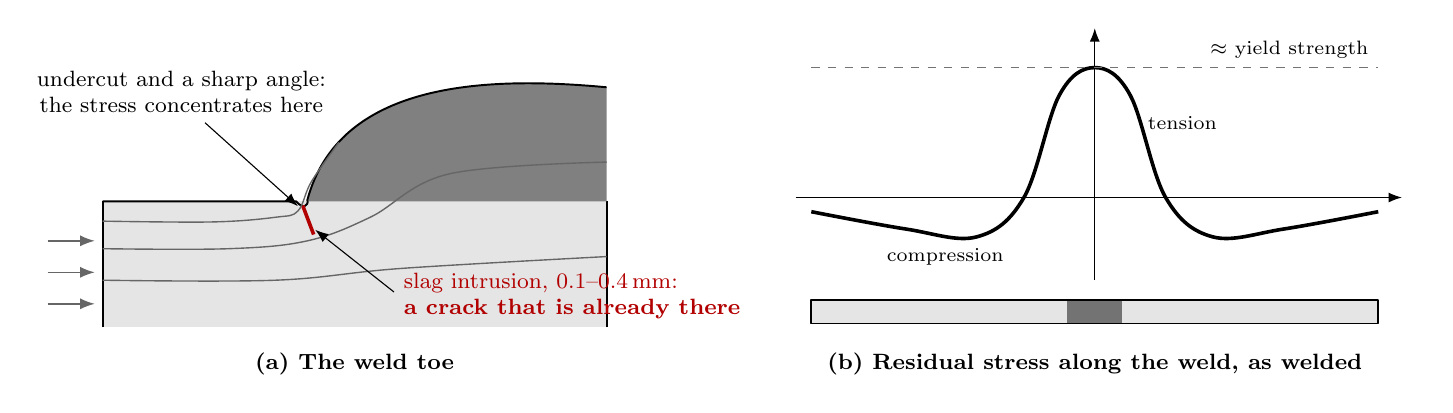
\begin{tikzpicture}[>=Latex,line join=round]
\tikzset{lab/.style={font=\footnotesize}, sm/.style={font=\scriptsize}}
% ---- (a) the toe ----
\begin{scope}
\fill[black!10] (-3.2,-1.6) rectangle (3.2,0); \draw[line width=0.7pt] (-3.2,-1.6) -- (-3.2,0) (3.2,-1.6) -- (3.2,0);
\fill[black!50] (-0.6,0) .. controls (-0.2,1.5) and (1.6,1.6) .. (3.2,1.45) -- (3.2,0) -- cycle;
\draw[line width=0.7pt] (-3.2,0) -- (-0.74,0) .. controls (-0.66,-0.1) and (-0.58,-0.06) .. (-0.6,0.02) .. controls (-0.2,1.5) and (1.6,1.6) .. (3.2,1.45);
\draw[red!70!black,line width=1.3pt] (-0.66,-0.05) -- (-0.52,-0.42);
\foreach \y/\s in {-0.5/0,-0.9/0,-1.3/0}{\draw[->,black!60,line width=0.5pt] (-3.9,\y) -- (-3.3,\y);}
\draw[black!60,line width=0.5pt] plot[smooth,tension=0.6] coordinates {(-3.2,-0.25) (-1.8,-0.26) (-1.0,-0.2) (-0.72,-0.12) (-0.55,0.25) (-0.2,0.75)};
\draw[black!60,line width=0.5pt] plot[smooth,tension=0.6] coordinates {(-3.2,-0.6) (-1.6,-0.6) (-0.6,-0.5) (0.2,-0.2) (1.2,0.35) (3.2,0.5)};
\draw[black!60,line width=0.5pt] plot[smooth,tension=0.6] coordinates {(-3.2,-1.0) (-1.0,-1.0) (0.6,-0.85) (3.2,-0.7)};
\draw[<-,line width=0.4pt] (-0.72,-0.06) -- (-1.9,1.0); \node[lab,anchor=south,align=center] at (-2.2,1.0) {undercut and a sharp angle:\\ the stress concentrates here};
\draw[<-,line width=0.4pt] (-0.5,-0.36) -- (0.5,-1.15); \node[lab,anchor=west,align=left,text=red!70!black] at (0.5,-1.2) {slag intrusion, 0.1--\SI{0.4}{mm}:\\ \textbf{a crack that is already there}};
\node[lab,anchor=north] at (0,-1.8) {\textbf{(a) The weld toe}};
\end{scope}
% ---- (b) residual stress across a butt weld ----
\begin{scope}[xshift=9.4cm,yshift=-0.55cm]
\fill[black!10] (-3.6,-1.0) rectangle (3.6,-0.7); \fill[black!55] (-0.35,-1.0) rectangle (0.35,-0.7); \draw[line width=0.6pt] (-3.6,-1.0) rectangle (3.6,-0.7);
\draw[->] (-3.8,0.6) -- (3.9,0.6); \draw[->] (0,-0.45) -- (0,2.75);
\draw[line width=1.3pt] plot[smooth,tension=0.6] coordinates {(-3.6,0.42) (-2.4,0.2) (-1.5,0.1) (-0.9,0.6) (-0.45,1.9) (0,2.25) (0.45,1.9) (0.9,0.6) (1.5,0.1) (2.4,0.2) (3.6,0.42)};
\draw[dashed,black!55,line width=0.4pt] (-3.6,2.25) -- (3.6,2.25); \node[sm,anchor=south east] at (3.6,2.25) {$\approx$ yield strength};
\node[sm,anchor=west] at (0.55,1.55) {tension}; \node[sm,anchor=north] at (-1.9,0.08) {compression};
\node[sm,anchor=west] at (3.95,0.6) {};
\node[lab,anchor=north] at (0,-1.25) {\textbf{(b) Residual stress along the weld, as welded}};
\end{scope}
\end{tikzpicture}
}
\end{frame}

\begin{frame}{Why Lectures 2 to 4 do not transfer directly}
\begin{enumerate}
  \item \textbf{There is no initiation phase.} The toe carries intrusions a few tenths of a
        millimetre deep. Lecture 3 called that an initial crack. Life is \alert{crack growth from
        the first cycle} --- hence an S--N slope of 3, the Paris exponent.
  \item \textbf{Stronger steel does not help.} Crack growth rate hardly depends on strength. The
        same joint in a \SI{700}{MPa} steel and a \SI{350}{MPa} steel has the \alert{same life}.
  \item \textbf{The mean stress is already at yield.} Residual tension near yield at the toe: every
        cycle runs from yield downward. The applied mean stops mattering.
\end{enumerate}
\vfill
So welded fatigue data is written in \alert{stress range} $\Delta\sigma$ --- with no Goodman correction.
\end{frame}

\begin{frame}{Detail categories}
\begin{columns}[c]
\begin{column}{0.4\textwidth}
Life depends on the \emph{geometry of the detail}, not the alloy. So details are classified.

\medskip
The class is a number: the stress range, in MPa, survived for $2\times10^{6}$ cycles.
\[ N=2\times10^{6}\left(\frac{\mathrm{FAT}}{\Delta\sigma}\right)^{3} \]
$\Delta\sigma$ is the \alert{nominal} range in the member. The weld's stress concentration is
already inside the class.
\end{column}
\begin{column}{0.6\textwidth}
\resizebox{\textwidth}{!}{% S-N curves for classified welded details (IIW, steel): stress range against cycles.
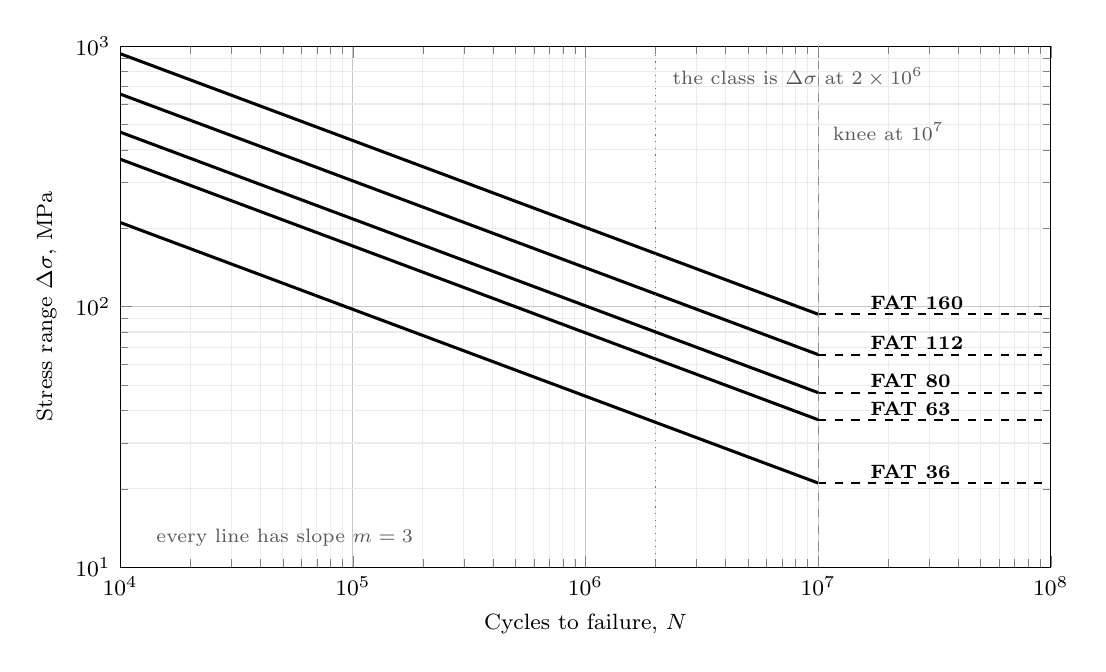
\begin{tikzpicture}
\begin{loglogaxis}[width=13.4cm,height=8.2cm,xmin=1e4,xmax=1e8,ymin=10,ymax=1000,
  xlabel={Cycles to failure, $N$},ylabel={Stress range $\Delta\sigma$, MPa},
  label style={font=\footnotesize},tick label style={font=\footnotesize},grid=both,
  major grid style={black!22},minor grid style={black!8},clip=true]
% FAT lines: N = 2e6 (FAT/ds)^3 down to the knee at 1e7, then flat
\addplot[black,line width=1.1pt,domain=1e4:1e7,samples=2] {160*(2e6/x)^(1/3)};
\addplot[black,line width=0.7pt,dashed,domain=1e7:1e8,samples=2] {93.57};
\addplot[black,line width=1.1pt,domain=1e4:1e7,samples=2] {112*(2e6/x)^(1/3)};
\addplot[black,line width=0.7pt,dashed,domain=1e7:1e8,samples=2] {65.50};
\addplot[black,line width=1.1pt,domain=1e4:1e7,samples=2] {80*(2e6/x)^(1/3)};
\addplot[black,line width=0.7pt,dashed,domain=1e7:1e8,samples=2] {46.78};
\addplot[black,line width=1.1pt,domain=1e4:1e7,samples=2] {63*(2e6/x)^(1/3)};
\addplot[black,line width=0.7pt,dashed,domain=1e7:1e8,samples=2] {36.84};
\addplot[black,line width=1.1pt,domain=1e4:1e7,samples=2] {36*(2e6/x)^(1/3)};
\addplot[black,line width=0.7pt,dashed,domain=1e7:1e8,samples=2] {21.05};
\addplot[black!55,line width=0.4pt,dotted] coordinates {(2e6,10) (2e6,1000)};
\node[font=\scriptsize,anchor=south west,text=black!65] at (axis cs:2.15e6,640) {the class is $\Delta\sigma$ at $2\times10^{6}$};
\node[font=\scriptsize\bfseries,anchor=south west,inner sep=1.5pt] at (axis cs:1.6e7,93.6) {FAT 160};
\node[font=\scriptsize\bfseries,anchor=south west,inner sep=1.5pt] at (axis cs:1.6e7,65.5) {FAT 112};
\node[font=\scriptsize\bfseries,anchor=south west,inner sep=1.5pt] at (axis cs:1.6e7,46.8) {FAT 80};
\node[font=\scriptsize\bfseries,anchor=south west,inner sep=1.5pt] at (axis cs:1.6e7,36.8) {FAT 63};
\node[font=\scriptsize\bfseries,anchor=south west,inner sep=1.5pt] at (axis cs:1.6e7,21.05) {FAT 36};
\node[font=\scriptsize,anchor=south west,text=black!65] at (axis cs:1.05e7,400) {knee at $10^{7}$};
\draw[black!45,line width=0.3pt,dashed] (axis cs:1e7,10) -- (axis cs:1e7,1000);
\node[font=\scriptsize,anchor=south west,text=black!65] at (axis cs:1.3e4,11) {every line has slope $m=3$};
\end{loglogaxis}
\end{tikzpicture}
}
\end{column}
\end{columns}
\end{frame}

\begin{frame}{The classes worth remembering}
\centering\small
\begin{tabular}{@{}lcc@{}}
\toprule
\textbf{Detail} & \textbf{Steel} & \textbf{Aluminium}\\
\midrule
Plain rolled plate or extrusion, no weld & 160 & 71\\
Transverse butt weld, ground flush, fully inspected & 112 & 45\\
Transverse butt weld, as welded, good shop quality & 90 & 36\\
Transverse butt weld, as welded, ordinary quality & 80 & 32\\
Plate with a fillet-welded attachment across it (carries no load) & 80 & 28\\
Cruciform joint, load-carrying fillets --- crack from the toe & 63 & 22\\
End of a long cover plate welded to a flange & 45--56 & 16--20\\
Cruciform joint, load-carrying fillets --- crack from the root & 36 & 12\\
\bottomrule
\end{tabular}

\vfill\raggedright\normalsize
\begin{itemize}
  \item Merely \alert{attaching} something halves the class.
  \item A load-carrying fillet can fail from the \alert{root} --- unseen --- at under a quarter of plain plate.
  \item Aluminium is about a third of steel: the ratio of the moduli.
\end{itemize}
{\footnotesize IIW Recommendations (Hobbacher).}
\end{frame}

\begin{frame}{Example 7.4 --- a bracket welded to a tension member}
$100\times\SI{10}{mm}$ flat, load cycling 0 to \SI{120}{kN}: \ $\Delta\sigma=\SI{120}{MPa}$. Bracket carries no load: FAT 80.
\[ N=2\times10^{6}\left(\tfrac{80}{120}\right)^{3}=5.9\times10^{5}\ \text{cycles} \]
\centering\small
\begin{tabular}{@{}lll@{}}
\toprule
Change one thing & Class & Life, cycles\\
\midrule
As drawn & 80 & $5.9\times10^{5}$\\
Steel changed to a \SI{700}{MPa} grade & 80 & $5.9\times10^{5}$ --- \alert{no change}\\
Toes ground to a smooth blend & 100 & $1.2\times10^{6}$\\
Bracket removed and bolted on elsewhere & 160 & $4.7\times10^{6}$\\
Bracket made to carry load through its fillets & 63 & $2.9\times10^{5}$\\
\ldots and under-sized, so it cracks from the root & 36 & $5.4\times10^{4}$\\
\bottomrule
\end{tabular}
\end{frame}

\begin{frame}{The same detail by the method of Lecture 2}
Shigley: $K_f=1.5$ at the toe of a transverse fillet.

\medskip
S355, $S_{ut}=\SI{510}{MPa}$, as-forged surface: $k_a=272(510)^{-0.995}=0.55$; axial, $k_c=0.85$:
\[ S_e=0.55\times0.85\times255=\SI{119}{MPa} \]
$\sigma_a=\sigma_m=1.5\times60=\SI{90}{MPa}$ \ $\Rightarrow$ \ Goodman: $n=1.07$ --- \emph{infinite life, just}.

\vfill
The classification said \num{590000} cycles.

\begin{alertblock}{Believe the classification}
It is built on tests of real welded details, with their flaws and their residual stress. The
stress-concentration method knows about neither.
\end{alertblock}
{\footnotesize For the \SI{700}{MPa} steel $k_a$ falls to 0.37 and $S_e$ is again \SI{119}{MPa}: the surface factor already tells half the story.}
\end{frame}

\begin{frame}{Shigley's fatigue factors --- for ranking}
\begin{columns}[c]
\begin{column}{0.45\textwidth}
\centering
\begin{tabular}{@{}lc@{}}
\toprule
\textbf{Weld} & $K_{fs}$\\
\midrule
Reinforced butt weld & 1.2\\
Toe of a transverse fillet & 1.5\\
End of a parallel fillet & \alert{2.7}\\
T-butt, sharp corners & 2.0\\
\bottomrule
\end{tabular}

\medskip{\footnotesize Shigley, Table 9--5}
\end{column}
\begin{column}{0.5\textwidth}
Useful for a first estimate, and they carry the right message:

\medskip
the \alert{end of a parallel fillet} is the worst place on a welded joint.

\medskip
For a life prediction on anything that matters, use a detail category.
\end{column}
\end{columns}
\end{frame}

\begin{frame}{Making a weld better in fatigue}
The toe is the problem, so every method works on the toe.
\begin{itemize}
  \item \textbf{Change the geometry.} Grind the toe to a blend, or remelt it with a TIG torch.
        About $\times1.3$ on the class --- more than double the life.
  \item \textbf{Change the residual stress.} Hammer or needle peening: $\times1.3$ to $1.5$.
        Furnace stress relief removes the tension but leaves the notch.
  \item \textbf{Change the weld type.} A ground-flush butt is class 112. No fillet reaches it.
  \item \textbf{Move the weld.} \alert{The cheapest of all}: put it where the stress range is low.
\end{itemize}
\end{frame}

\section{Defects, inspection, the special process}

\begin{frame}{What can be wrong with a weld}
\centering
\resizebox{0.8\textwidth}{!}{% What can be wrong with a weld, in one section.
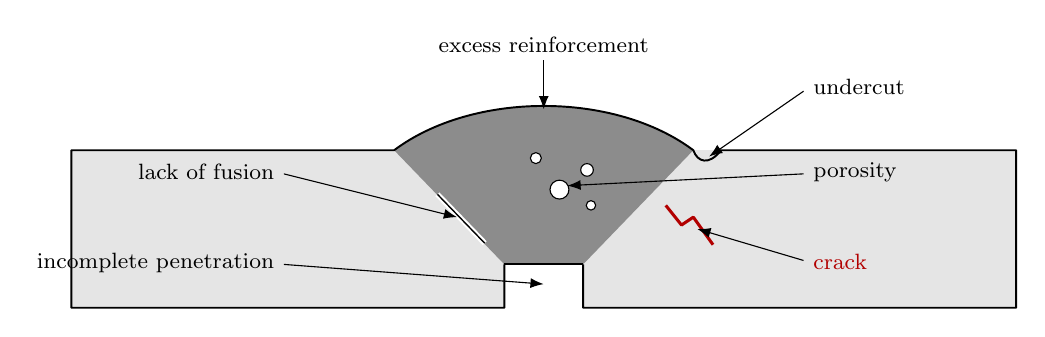
\begin{tikzpicture}[>=Latex,line join=round]
\tikzset{lab/.style={font=\footnotesize}}
\fill[black!10] (-6,0) rectangle (6,2); 
\fill[black!45] (-0.5,0.55) -- (-1.9,2) .. controls (-0.9,2.75) and (0.9,2.75) .. (1.9,2) -- (0.5,0.55) -- cycle;
\fill[white] (-0.5,0) rectangle (0.5,0.55);
\draw[line width=0.7pt] (0.5,0.55) -- (0.5,0) -- (6,0) -- (6,2) -- (2.25,2) .. controls (2.1,1.8) and (1.95,1.85) .. (1.9,2) .. controls (0.9,2.75) and (-0.9,2.75) .. (-1.9,2) -- (-6,2) -- (-6,0) -- (-0.5,0) -- (-0.5,0.55);
\draw[line width=0.7pt] (-0.5,0.55) -- (0.5,0.55);
% porosity
\foreach \x/\y/\r in {0.2/1.5/0.12,0.55/1.75/0.08,-0.1/1.9/0.07,0.6/1.3/0.06}{\fill[white] (\x,\y) circle[radius=\r]; \draw[line width=0.4pt] (\x,\y) circle[radius=\r];}
% lack of fusion on the left wall
\draw[white,line width=2pt] (-0.75,0.82) -- (-1.35,1.44); \draw[line width=0.5pt] (-0.75,0.82) -- (-1.35,1.44);
% crack in HAZ, right
\draw[red!70!black,line width=1.1pt] (1.55,1.3) -- (1.75,1.05) -- (1.9,1.15) -- (2.15,0.8);
% callouts
\draw[<-,line width=0.4pt] (2.1,1.92) -- (3.3,2.75); \node[lab,anchor=west] at (3.3,2.8) {undercut};
\draw[<-,line width=0.4pt] (0,2.52) -- (0,3.15); \node[lab,anchor=south] at (0,3.12) {excess reinforcement};
\draw[<-,line width=0.4pt] (0.3,1.55) -- (3.3,1.7); \node[lab,anchor=west] at (3.3,1.72) {porosity};
\draw[<-,line width=0.4pt] (-1.1,1.15) -- (-3.3,1.7); \node[lab,anchor=east] at (-3.3,1.72) {lack of fusion};
\draw[<-,line width=0.4pt] (0,0.3) -- (-3.3,0.55); \node[lab,anchor=east] at (-3.3,0.57) {incomplete penetration};
\draw[<-,line width=0.4pt] (1.95,1.0) -- (3.3,0.6); \node[lab,anchor=west,text=red!70!black] at (3.3,0.58) {crack};
\end{tikzpicture}
}

\vfill\raggedright
The \alert{planar} defects --- cracks, lack of fusion, incomplete penetration --- are the dangerous
ones. They are cracks, and Lecture 3 applies to them directly.
\end{frame}

\begin{frame}{Which inspection finds which defect}
\centering\footnotesize
\begin{tabular}{@{}lll@{}}
\toprule
\textbf{Defect} & \textbf{What it is} & \textbf{Found by}\\
\midrule
Crack & hot (freezing) or cold (hydrogen, hard HAZ, hours later) & penetrant, magnetic particle, ultrasonic\\
Lack of fusion & weld metal lying on the wall, not bonded & ultrasonic; radiography only if well oriented\\
Incomplete penetration & the root never melted & radiography, ultrasonic\\
Porosity & trapped gas & radiography\\
Undercut & groove melted into the parent at the toe & visual, gauge\\
Excess reinforcement & too much bead: a sharper toe & visual, gauge\\
\bottomrule
\end{tabular}

\vfill\raggedright\normalsize
Radiography is good at volumes and poor at tight planar flaws.

\alert{The defects that matter most are the ones the most familiar method is worst at.}
\end{frame}

\begin{frame}{Welding is a special process}
A hole can be gauged. A weld cannot be proven sound from the finished part. So quality is
controlled \alert{before and during} the weld:
\begin{enumerate}
  \item a \textbf{welding procedure specification} --- process, filler, preparation, heat input,
        pre- and post-weld treatment --- proven by breaking a sample joint;
  \item a \textbf{qualified welder}, tested on that procedure, and re-tested;
  \item an \textbf{inspection class} on the drawing. AWS D17.1: classes A, B, C --- class A is a
        weld whose failure loses the aircraft.
\end{enumerate}
\vfill
This is what ``approved practices'' meant.

A weld callout is not complete with a size: it needs \alert{process, filler, class, inspection,
post-weld treatment}.
\end{frame}

\section{Where to put a weld}

\begin{frame}{Construction: where to put a weld (1)}
\begin{enumerate}
  \item \textbf{Where the stress is low.} Near the neutral axis, away from maximum moment.
        Lecture 1's error 6 is this rule broken.
  \item \textbf{Do not weld an attachment to a highly stressed member} if you can clamp or bolt it.
  \item \textbf{Butt before fillet, continuous before intermittent,} where the load cycles. Every
        start and stop is a toe.
  \item \textbf{Keep weld ends out of corners} and away from changes of section.
  \item \textbf{Do not let welds cross or pile up.} Stop one short, or cut a clearance hole.
\end{enumerate}
\end{frame}

\begin{frame}{Construction: where to put a weld (2)}
\begin{enumerate}\setcounter{enumi}{5}
  \item \textbf{Give the torch and the inspector room.} What cannot be reached is made badly; what
        cannot be seen is not inspected.
  \item \textbf{Balance the welding about the neutral axis.} Weld metal shrinks; an unbalanced weld
        distorts the part and leaves it stressed.
  \item \textbf{Never weld on a part heat treated for strength without heat treating it again.} Nor
        near a thread, a bearing seat or a ground surface. A tack counts. So does a
        \alert{stray arc strike}.
  \item \textbf{On steel tube, scarf or fishmouth the ends,} and use gussets to spread a cluster.
\end{enumerate}
\end{frame}

\begin{frame}{What to take away}
\begin{enumerate}
  \item Three questions: the weld metal, the parent beside it, the toe.
  \item Steel gets a hard HAZ, heat-treated aluminium a soft one. Re-heat-treat, or design to the welded strength.
  \item Fillets: $\tau=F/(0.707\,h\,l)$, whatever the direction. Check the parent too.
  \item Say throat or leg on the drawing.
  \item 4130 tube: use the welded allowable, cut the ends at $30^\circ$.
  \item Fatigue: stress range and a detail category. Stronger steel does not help.
  \item The cheapest improvement is to move the weld; the next is to grind the toe.
  \item Specify the process, not just the size.
\end{enumerate}
\vfill
\emph{Next:} welds in groups under bending and torsion --- and adhesive bonding.
\end{frame}

\end{document}
